\documentclass[12pt,a4paper]{article}
\usepackage[margin=2.3cm]{geometry}
\usepackage[T1]{fontenc}
\usepackage{mathpazo}
\usepackage{amsmath,amssymb}
\usepackage{tikz}
\usepackage{enumitem}
\setlength{\parindent}{0pt}
\setlength{\parskip}{6pt}
\setlist{itemsep=1pt,topsep=2pt}
\pagestyle{plain}
\newcommand{\Ahat}{\hat A}
\newcommand{\R}{\mathbb{R}}
\newcommand{\h}[1]{\par\medskip\textbf{\large #1}\par}

\begin{document}

\begin{center}
{\Large\bfseries Vanilla GCN}\\[2pt]
{\large Mathematical Modelling}\\[6pt]
[Your name] \quad [Roll no.]
\end{center}

Detecting illicit Bitcoin transactions on the Elliptic dataset using a 2-layer Vanilla GCN.

%==============================================================
\section*{Part 1: The Model}

\h{Graph Representation}
\[
  G = (V, E), \qquad |V| = 203{,}769 \ (\text{transactions}), \qquad |E| = 234{,}355 \ (\text{money flows})
\]
Adjacency matrix: \quad $A \in \{0,1\}^{N\times N}$

Feature matrix: \quad $X \in \R^{N\times F}$, \quad $F = 165$

Label: \quad $y \in \{0, 1\}$, \quad $0 = $ licit, \ $1 = $ illicit

\h{Symmetric Normalisation of the Adjacency Matrix}
Self-loops: \quad $\tilde A = A + I_N$

Degree matrix: \quad $\tilde D_{ii} = \sum_j \tilde A_{ij}$

Symmetric normalisation: \quad $\Ahat = \tilde D^{-1/2}\, \tilde A\, \tilde D^{-1/2}$

$A$ alone gives unequal scale to high- and low-degree nodes. Symmetric normalisation gives a fair weighted average and
keeps the edge weight equal in both directions.

\h{Feature Normalisation}
\[
  x_{ij} \leftarrow \frac{x_{ij} - \mu_j}{\sigma_j}
\]
($\mu_j$ = mean, $\sigma_j$ = standard deviation of feature $j$)

\h{GCN Layer and Forward Pass}
\[
  H^{(l+1)} = \sigma\big(\Ahat\, H^{(l)}\, W^{(l)}\big)
\]
$H^{(l)} \in \R^{N\times d_l}$ $\rightarrow$ node features entering layer $l$

$W^{(l)} \in \R^{d_l\times d_{l+1}}$ $\rightarrow$ learnable weight matrix

$\Ahat$ $\rightarrow$ normalised adjacency matrix

$\sigma$ $\rightarrow$ activation (ReLU for the hidden layer)

\textbf{2-layer Vanilla GCN forward pass:}
\[
  Z = \mathrm{softmax}\Big(\Ahat\cdot \mathrm{ReLU}\big(\Ahat\cdot X\cdot W^{(0)}\big)\cdot W^{(1)}\Big)
\]
$N = 203{,}769$ \qquad $F = 165$ \qquad $H = 100$ hidden \qquad $C = 2$ classes

\begin{tabular}{@{}l@{\quad}l@{\hspace{1.5cm}}l}
$X$ & $\rightarrow N\times F$ & $XW$ $\rightarrow$ linear transformation\\
$XW^{(0)}$ & $\rightarrow N\times H$ & \phantom{$XW$ $\rightarrow$} of each node's own features\\
$H^{(1)} = \mathrm{ReLU}(\Ahat XW^{(0)})$ & $\rightarrow N\times H$ & $\Ahat(\cdot)$ $\rightarrow$ aggregation\\
$H^{(1)}W^{(1)}$ & $\rightarrow N\times C$ & $\sigma(\cdot)$ $\rightarrow$ non-linearity (ReLU)\\
$\Ahat(H^{(1)}W^{(1)}) = Z$ & $\rightarrow N\times C$ &
\end{tabular}

\h{Loss Function}
Weighted cross-entropy loss, computed only over labelled training nodes. Illicit transactions are rare (about 10\%),
so they get a higher weight: $w_1 = 0.7$ (illicit), $w_0 = 0.3$ (licit).
\[
  \mathcal L = -\frac{1}{\sum_{i\in V_{\text{train}}} w_{y_i}} \sum_{i\in V_{\text{train}}} w_{y_i}\, \log Z_{i, y_i}
\]

\h{Training Process}
Minimise $\mathcal L$ with respect to the weights $\theta = \{W^{(0)}, W^{(1)}\}$ using the Adam optimiser:
\[
  \theta \leftarrow \theta - \eta\cdot \text{Adam update}(\nabla_\theta \mathcal L), \qquad \eta = 0.01
\]
$\nabla_\theta\mathcal L$ $\rightarrow$ computed by backpropagation (chain rule).

\textbf{One training epoch:}
\begin{enumerate}
  \item Forward pass on the full graph $\rightarrow Z$
  \item Compute loss $\mathcal L$ on training nodes only
  \item Backward pass $\rightarrow$ compute $\nabla_\theta\mathcal L$
  \item Update weights (gradient descent step)
\end{enumerate}
Repeated for 200 epochs. We train on time steps 1--34 and test on time steps 35--49 (future transactions).

\h{Evaluation Metrics}
On $V_{\text{test}}$ (illicit = positive class):
\[
  \text{Precision} = \frac{TP}{TP + FP} \qquad\quad \text{Recall} = \frac{TP}{TP + FN}
\]
\[
  F_1 = \frac{2\cdot\text{Precision}\cdot\text{Recall}}{\text{Precision} + \text{Recall}}
\]
Our result: \ $TP = 507$, \ $FP = 182$, \ $FN = 576$
\[
  \text{Precision} = \frac{507}{689} = 0.736, \qquad \text{Recall} = \frac{507}{1083} = 0.468, \qquad F_1 = 0.572
\]
Accuracy is not used because only about 6.5\% of test transactions are illicit. A model that always says ``licit''
would be 93.5\% accurate but would catch no criminal.

\newpage
%==============================================================
\section*{Part 2: Worked Example}

\h{1. Graph}
Let $V = \{0, 1, 2, 3, 4\}$ be five transactions.
\[
  E = \{(0,1),\ (1,2),\ (1,3),\ (2,3),\ (3,4)\}
\]
Money flows $0 \rightarrow 1 \rightarrow 2, 3 \rightarrow 4$.

\begin{center}
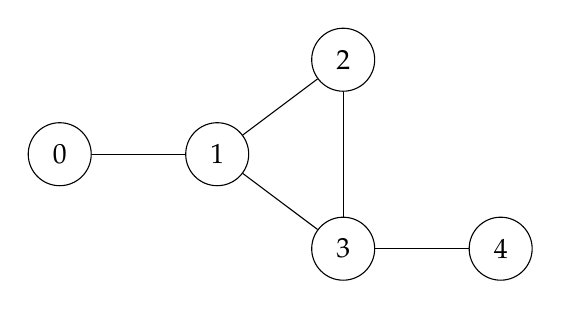
\begin{tikzpicture}[every node/.style={circle, draw, minimum size=8mm}]
  \node (0) at (0,0) {0};
  \node (1) at (2,0) {1};
  \node (2) at (3.6,1.2) {2};
  \node (3) at (3.6,-1.2) {3};
  \node (4) at (5.6,-1.2) {4};
  \draw (0)--(1); \draw (1)--(2); \draw (1)--(3); \draw (2)--(3); \draw (3)--(4);
\end{tikzpicture}
\end{center}

Adjacency matrix, degree vector, degree matrix:
\[
  A = \begin{bmatrix}
  0&1&0&0&0\\ 1&0&1&1&0\\ 0&1&0&1&0\\ 0&1&1&0&1\\ 0&0&0&1&0
  \end{bmatrix}, \qquad d = [1, 3, 2, 3, 1], \qquad D = \mathrm{diag}(1, 3, 2, 3, 1)
\]

\h{2. Add Self-Loops}
\[
  \tilde A = A + I = \begin{bmatrix}
  1&1&0&0&0\\ 1&1&1&1&0\\ 0&1&1&1&0\\ 0&1&1&1&1\\ 0&0&0&1&1
  \end{bmatrix}
  \begin{matrix} =2\\=4\\=3\\=4\\=2 \end{matrix}
  \qquad \tilde D = \mathrm{diag}(2, 4, 3, 4, 2)
\]

\h{3. Symmetric Normalisation}
\[
  \tilde D^{-1/2} = \mathrm{diag}\Big(\frac{1}{\sqrt2},\ \frac12,\ \frac{1}{\sqrt3},\ \frac12,\ \frac{1}{\sqrt2}\Big)
\]
Using $\Ahat = \tilde D^{-1/2}\tilde A\tilde D^{-1/2}$, \ entrywise $\Ahat_{ij} = \dfrac{\tilde A_{ij}}{\sqrt{\tilde d_i \tilde d_j}}$:
\[
  \Ahat = \begin{bmatrix}
  \frac12 & \frac{1}{2\sqrt2} & 0 & 0 & 0\\[3pt]
  \frac{1}{2\sqrt2} & \frac14 & \frac{1}{2\sqrt3} & \frac14 & 0\\[3pt]
  0 & \frac{1}{2\sqrt3} & \frac13 & \frac{1}{2\sqrt3} & 0\\[3pt]
  0 & \frac14 & \frac{1}{2\sqrt3} & \frac14 & \frac{1}{2\sqrt2}\\[3pt]
  0&0&0&\frac{1}{2\sqrt2} & \frac12
  \end{bmatrix}
  \approx
  \begin{bmatrix}
  0.5 & 0.354 & 0 & 0 & 0\\
  0.354 & 0.25 & 0.289 & 0.25 & 0\\
  0 & 0.289 & 0.333 & 0.289 & 0\\
  0 & 0.25 & 0.289 & 0.25 & 0.354\\
  0 & 0 & 0 & 0.354 & 0.5
  \end{bmatrix}
\]
($\Ahat$ is symmetric, as required, since $\tilde A$ and $\tilde D$ are symmetric.)

\h{4. Feature Matrix}
Two features per transaction, $X \in \R^{5\times2}$: \
$f_1$ = unusual output pattern, \ $f_2$ = normal fee pattern.
\[
  \begin{array}{c|cc}
  \text{Node} & f_1 & f_2\\ \hline
  0 & 1 & 0\\ 1 & 1 & 1\\ 2 & 1 & 0\\ 3 & 0 & 1\\ 4 & 0 & 1
  \end{array}
  \qquad\qquad
  X = H^{(0)} = \begin{bmatrix} 1&0\\ 1&1\\ 1&0\\ 0&1\\ 0&1 \end{bmatrix} \in \R^{5\times2}
\]

\h{5. Labels}
$C = 2$. Nodes 0 and 4 are labelled training nodes:

$y_0 = $ class 1 (illicit), \quad $y_4 = $ class 0 (licit)

One-hot: \ $y_0 = [0, 1]$, \ $y_4 = [1, 0]$. The remaining nodes are unlabelled during training. \ $V_L = \{0, 4\}$

\h{6. Vanilla GCN Propagation Rule}
\[
  H^{(k+1)} = \sigma\big(\Ahat H^{(k)} W^{(k)}\big)
\]
With $H^{(0)} = X$ and $W^{(0)} = I_2$ (identity: the first layer only mixes neighbourhoods, with no feature transform):
\[
  H^{(1)} = \mathrm{ReLU}(\Ahat X I) = \mathrm{ReLU}(\Ahat X)
\]
Computation of $H^{(1)} = \Ahat X$, \ $(\Ahat X)_{ij} = \sum_k \Ahat_{ik} X_{kj}$:
\begin{align*}
  H^{(1)}_0 &= \tfrac12(1,0) + \tfrac{1}{2\sqrt2}(1,1) = \Big(\tfrac12 + \tfrac{1}{2\sqrt2},\ \tfrac{1}{2\sqrt2}\Big)\\
  H^{(1)}_1 &= \tfrac{1}{2\sqrt2}(1,0) + \tfrac14(1,1) + \tfrac{1}{2\sqrt3}(1,0) + \tfrac14(0,1)
              = \Big(\tfrac{1}{2\sqrt2} + \tfrac14 + \tfrac{1}{2\sqrt3},\ \tfrac12\Big)\\
  H^{(1)}_2 &= \tfrac{1}{2\sqrt3}(1,1) + \tfrac13(1,0) + \tfrac{1}{2\sqrt3}(0,1) = \Big(\tfrac{1}{2\sqrt3} + \tfrac13,\ \tfrac{1}{\sqrt3}\Big)\\
  H^{(1)}_3 &= \tfrac14(1,1) + \tfrac{1}{2\sqrt3}(1,0) + \tfrac14(0,1) + \tfrac{1}{2\sqrt2}(0,1)
              = \Big(\tfrac14 + \tfrac{1}{2\sqrt3},\ \tfrac12 + \tfrac{1}{2\sqrt2}\Big)\\
  H^{(1)}_4 &= \tfrac{1}{2\sqrt2}(0,1) + \tfrac12(0,1) = \Big(0,\ \tfrac12 + \tfrac{1}{2\sqrt2}\Big)
\end{align*}
All values are $\ge 0$, so ReLU makes no changes.
\[
  H^{(1)} \approx \begin{bmatrix}
  0.854 & 0.354\\ 0.892 & 0.500\\ 0.622 & 0.577\\ 0.539 & 0.854\\ 0 & 0.854
  \end{bmatrix}
\]

\h{7. Output (Classification Layer)}
Take a second weight matrix so that the two scores are exact negatives of one another:
\[
  W^{(1)} = \begin{bmatrix} -1 & 1\\ 1 & -1 \end{bmatrix}, \qquad Z = \Ahat H^{(1)} W^{(1)}
\]
Compute in two stages: \ $M = \Ahat H^{(1)}$, then $Z = M W^{(1)}$.
\begin{align*}
  M_0 &= \tfrac12(0.854,\ 0.354) + \tfrac{1}{2\sqrt2}(0.892,\ 0.5) = (0.742,\ 0.354)\\
  M_4 &= \tfrac{1}{2\sqrt2}(0.539,\ 0.854) + \tfrac12(0,\ 0.854) = (0.190,\ 0.729)
\end{align*}
Doing the same for all rows:
\[
  M \approx \begin{bmatrix}
  0.742 & 0.354\\ 0.839 & 0.630\\ 0.620 & 0.583\\ 0.537 & 0.807\\ 0.190 & 0.729
  \end{bmatrix}
\]
$Z = M W^{(1)}$: each row satisfies $Z_{i0} = M_{i1} - M_{i0} = -Z_{i1}$.
\[
  Z \approx \begin{bmatrix}
  -0.389 & 0.389\\ -0.209 & 0.209\\ -0.037 & 0.037\\ 0.270 & -0.270\\ 0.538 & -0.538
  \end{bmatrix}
\]

\h{8. Softmax Reduces to a Sigmoid}
Because the two scores in every row are exact negatives, $Z_{i0} = -Z_{i1} = -z$, the two-class softmax is
\[
  P_{i1} = \frac{e^{z}}{e^{-z} + e^{z}} = \frac{1}{1 + e^{-2z}}
\]
which is a plain sigmoid of $2z$.

Labelled node 0 \ ($z = Z_{0,1} = 0.389$):
\[
  P_{0,1} = \frac{1}{1 + e^{-0.777}} = \frac{1}{1 + 0.460} \approx 0.685, \qquad P_{0,0} \approx 0.315
\]
\[
  P_0 \approx [0.315,\ 0.685] \quad \rightarrow \text{predicted illicit} \checkmark
\]
Labelled node 4 \ ($z = Z_{4,1} = -0.538$):
\[
  P_{4,1} = \frac{1}{1 + e^{1.076}} = \frac{1}{1 + 2.934} \approx 0.254, \qquad P_{4,0} \approx 0.746
\]
\[
  P_4 \approx [0.746,\ 0.254] \quad \rightarrow \text{predicted licit} \checkmark
\]
Unlabelled node 1 gets $P_1 \approx [0.397,\ 0.603]$, so it is flagged as illicit because it receives money from the illicit node 0.

\h{9. Cross-Entropy Loss}
\[
  \mathcal L = -\frac{1}{|V_L|}\sum_{i\in V_L}\sum_{c} y_{ic}\log P_{ic} = \frac12\big[-\log P_{0,1} - \log P_{4,0}\big]
\]
\[
  y_0 = [0, 1]: \quad \ell_0 = -\log(0.685) \approx 0.378
\]
\[
  y_4 = [1, 0]: \quad \ell_4 = -\log(0.746) \approx 0.293
\]
\[
  \mathcal L = \frac{0.378 + 0.293}{2} \approx \underline{\underline{0.336}}
\]

\h{10. Gradient of the Softmax Cross-Entropy}
\[
  P_{ic} = \frac{e^{Z_{ic}}}{\sum_{c'} e^{Z_{ic'}}} \qquad \ell_i = -\sum_c y_{ic}\log P_{ic}
\]
\[
  \frac{\partial P_{ic}}{\partial Z_{ic}} = P_{ic}(1 - P_{ic}), \qquad \frac{\partial P_{ic}}{\partial Z_{id}} = -P_{ic}P_{id} \quad (c \ne d)
\]
Combining:
\[
  \frac{\partial \ell_i}{\partial Z_{ic}} = P_{ic} - y_{ic}
\]
For node 0: \quad $\dfrac{\partial \ell_0}{\partial Z_{0,0}} = 0.315 - 0 = 0.315$, \qquad $\dfrac{\partial \ell_0}{\partial Z_{0,1}} = 0.685 - 1 = -0.315$

For node 4: \quad $\dfrac{\partial \ell_4}{\partial Z_{4,0}} = 0.746 - 1 = -0.254$, \qquad $\dfrac{\partial \ell_4}{\partial Z_{4,1}} = 0.254 - 0 = 0.254$

\h{11. Backpropagation to $\partial\mathcal L / \partial W^{(1)}$}
With $\mathcal L = \frac12(\ell_0 + \ell_4)$, only labelled rows carry a gradient $\frac12(P_i - y_i)$; unlabelled rows are 0.
\[
  dZ = \begin{bmatrix}
  0.157 & -0.157\\ 0&0\\ 0&0\\ 0&0\\ -0.127 & 0.127
  \end{bmatrix}
\]
Gradient with respect to $W^{(1)}$: since $Z = MW^{(1)}$, \ $\dfrac{\partial\mathcal L}{\partial W^{(1)}} = M^T dZ = M_0^T dZ_0 + M_4^T dZ_4$
\[
  \frac{\partial\mathcal L}{\partial W^{(1)}} \approx \begin{bmatrix} 0.093 & -0.093\\ -0.037 & 0.037 \end{bmatrix}
\]
A gradient descent step
\[
  W^{(k)} \leftarrow W^{(k)} - \eta\,\frac{\partial\mathcal L}{\partial W^{(k)}}
\]
completes one full training iteration of the Vanilla GCN.

\end{document}
